\section{Comparison between PREFLEX and TEXCP}
\begin{comment}

{\bf Balancing by path utilization}
\\In this section we consider a simplified version of TEXCP (the same as in 5.1.1) that balances path utilization but doesn't activate TEXCP congestion management measures and only balance the path utilization. As expected (figure \ref{fig:st-util}), the modified version do very well in equalizing the path utilization, achieving very quickly to changes in network traffic state while keeping a stable behaviour. 

However, by looking at the drop rate in bottlenecks (figure \ref{fig:st-drop}) we observe that it is not equal on the different links. This observation, have a meaningful explanation behind. The high drop rate on the like is compensated by a higher load (received bytes over the capacity) so the utilization is equal on the three links. This means that using only this measure for balancing the load we risk to drive the network to a suboptimal state. The other observation is about the loss level that ingress routers see using LEX codepoint (figure \ref{fig:st-loss1}). All the three interfaces, which correspond to the links, have the same level. This is an expected result since TEXP use FLARE which doesn't guarantee that retransmissions follow the same path as the original packet. This have another result is that within few RTTs, TCP routines using different paths experience the congestion of each of them and hence they adapt their transmission rate to a combination of loss rate in each path that could be estimated as:

\begin{equation}
\rho = \sum_{i} x_{i}\cdot \rho_{i} 
\end{equation}

where, $\rho_{i}$ and $x_{i}$ are respectively the loss rate and the probability to take path $i$. But we should keep in mind that such high levels of path utilization aren't frequent in intra-domain TE, since not all the flows are elastic as it is the case in our scenario. For such cases, TEXCP defines a feedback mechanism to control congestion.

\begin{figure}[h]
\begin{center}

\epsfig{file=img/sec-5-2-3/no-traffic-shaper/util, width=4.5in}
\caption{
  The link utilization measured at the bottlenecks in simplified TEXCP.

   \label{fig:st-util}
}
\end{center}
\end{figure}

\begin{figure}[h]
\begin{center}

\epsfig{file=img/sec-5-2-3/no-traffic-shaper/dropRate, width=4.5in}
\caption{
  The drop rate measured at the bottlenecks in simplified TEXCP.

   \label{fig:st-drop}
}
\end{center}
\end{figure}

\begin{figure}[h]
\begin{center}

\epsfig{file=img/sec-5-2-3/no-traffic-shaper/10/throuputs, width=4.5in}
\caption{
  The throughput measured at ingress router I1 interfaces in simplified TEXCP.

   \label{fig:st-fwnd}
}
\end{center}
\end{figure}

\begin{figure}[h]
\begin{center}

\epsfig{file=img/sec-5-2-3/no-traffic-shaper/10/loss-192-0-0-0, width=4.5in}
\caption{
  Loss ratio $\rho_{i}$ for destination E1 as seen by balancer ingress router I1 in simplified TEXCP.

   \label{fig:st-loss1}
}
\end{center}
\end{figure}
\clearpage 

{\bf TEXCP}
\\In this section TEXCP was fully implemented. A traffic shaper is associated with each Ingress/Egress route and control the transmission rate over the different paths. The path utilization is still equalized for the three bottlenecks (figure \ref{fig:t-util}), but most importantly the difference in drop rate at each link disappeared (\ref{fig:t-drop}). The path utilization has slightly increased, which is correlated with the decrease in the drop rate at the bottleneck since TCP routing under low loss rate have a stable transmission rate and doesn't fluctuate a lot. By limiting the transmission rate, the effect of the traffic shaper is to move congestion and more precisely the dropping from the core network to the edge. 

The introduction of traffic shapers changes the loss rate. Indeed, traffic shaper allocates a buffer for each destination instead of the common buffer at the bottleneck. In our topology each link pass through the traffic of four IE pairs. Using traffic shapers means that four queues will be added. The number of added queues and their size are new parameters that influences the level of congestion. For instance the ratio buffer size over the transmission rate could decrease significantly the global loss rate if set to a high value, and the inverse is true. The mathematical formalization of this problem is quite difficult.

But the drawback of the use traffic shaping and transmission rate control, is to equally distributed bandwidth over pairs without considering the real amount of traffic travelling between them. Bandwidth waste is a known result of traffic shapping. But since we are using elastic flow the bandwidth is fully used, yet the level of loss is different from a destination to another (figure \ref{fig:t-loss1} and \ref{fig:t-loss2}). Starting from the moment when the bottlenecks feel congested, the transmission rate of each pair and path is decreased. The decrease mechanism is multiplicative, so if the transmission rates were defined equally at the beginning they will reach the same equilibrium. This is fine while they have equal number of flows but once this distribution change the different flows will keep having equal rates. This means that the level of congestion experience for one destination is different from another even if they share the same bottleneck. Hence the use of traffic shapers introduce unfairness.

\begin{figure}[h]
\begin{center}

\epsfig{file=img/sec-5-2-3/trafficShaper/util, width=4.5in}
\caption{
  The link utilization measured at the bottlenecks in TEXCP.

   \label{fig:t-util}
}
\end{center}
\end{figure}

\begin{figure}[h]
\begin{center}

\epsfig{file=img/sec-5-2-3/trafficShaper/dropRate, width=4.5in}
\caption{
  The drop rate measured at the bottlenecks in TEXCP.

   \label{fig:t-drop}
}
\end{center}
\end{figure}

\begin{figure}[h]
\begin{center}

\epsfig{file=img/sec-5-2-3/trafficShaper/10/throuputs, width=4.5in}
\caption{
  The throughput measured at ingress router I1 interfaces in TEXCP.

   \label{fig:t-fwnd}
}
\end{center}
\end{figure}

\begin{figure}[h]
\begin{center}

\epsfig{file=img/sec-5-2-3/trafficShaper/10/loss-192-0-0-0, width=4.5in}
\caption{
  Loss ratio $\rho_{i}$ for destination E1 as seen by balancer ingress router I1 in TEXCP.

   \label{fig:t-loss1}
}
\end{center}
\end{figure}

\begin{figure}[h]
\begin{center}

\epsfig{file=img/sec-5-2-3/trafficShaper/10/loss-192-0-1-0, width=4.5in}
\caption{
  Loss ratio $\rho_{i}$ for destination E2 as seen by balancer ingress router I1 in TEXCP.

   \label{fig:t-loss2}
}
\end{center}
\end{figure}

\clearpage 

{\bf PREFLEX}
\\ In this section a comparison is carried out with congestion balancing in PREFLEX. The congestion parameters of the balancing algorithm were set to : $\beta_{E}=0.9$, $\beta_{C}=0$ and $\beta_{L}=0.1$.

PREFLEX performance in balancing congestion is similar to the one obtained in the previous section for the same configuration (Analysis of PREFLEX balancing algorithm 5.2.2). 


\begin{figure}[h]
\begin{center}

\epsfig{file=img/sec-5-2-3/split-90-0-10/util, width=4.5in}
\caption{
  The link utilization measured at the bottlenecks in TEXCP.

   \label{fig:p-util}
}
\end{center}
\end{figure}

\begin{figure}[h]
\begin{center}

\epsfig{file=img/sec-5-2-3/split-90-0-10/dropRate, width=4.5in}
\caption{
  The drop rate measured at the bottlenecks in TEXCP.

   \label{fig:p-drop}
}
\end{center}
\end{figure}

\begin{figure}[h]
\begin{center}

\epsfig{file=img/sec-5-2-3/split-90-0-10/10/throuputs, width=4.5in}
\caption{
  The throughput measured at ingress router I1 interfaces in TEXCP.

   \label{fig:p-fwnd}
}
\end{center}
\end{figure}

\begin{figure}[h]
\begin{center}

\epsfig{file=img/sec-5-2-3/split-90-0-10/10/loss-192-0-0-0, width=4.5in}
\caption{
  Loss ratio $\rho_{i}$ for destination E1 as seen by balancer ingress router I1 in TEXCP.

   \label{fig:p-loss1}
}
\end{center}
\end{figure}

\begin{figure}[h]
\begin{center}

\epsfig{file=img/sec-5-2-3/split-90-0-10/10/loss-192-0-1-0, width=4.5in}
\caption{
  Loss ratio $\rho_{i}$ for destination E2 as seen by balancer ingress router I1 in PREFLEX.

   \label{fig:p-loss2}
}
\end{center}
\end{figure}
\end{comment}
